\documentclass[12pt, twoside]{report}
\usepackage[utf8]{inputenc}
\usepackage{titlesec}
\usepackage{geometry}
\usepackage{etoolbox}
\usepackage{xcolor}
\usepackage{enumitem}
\usepackage{amsmath}
\usepackage{amssymb}
\usepackage{xstring}
\usepackage{multicol}
\usepackage{tikz-dimline}
\usepackage{pdfpages}
\usepackage{setspace}

% To get current section name %
\usepackage{nameref}
\makeatletter
\newcommand*{\currentname}{\@currentlabelname}
\makeatother


% bibliography setup %
\usepackage[backend = biber,sorting = none]{biblatex}
\addbibresource{references.bib}


% On the spot flowchart creation %
\usetikzlibrary{shapes.geometric, arrows}
\tikzstyle{startstop} = [rectangle, rounded corners, minimum width=3cm, minimum height=1cm,text centered, draw=black, fill=red!30]
\tikzstyle{io} = [trapezium, trapezium left angle=70, trapezium right angle=110, minimum width=3cm, minimum height=1cm, text centered, draw=black, fill=blue!30]
\tikzstyle{process} = [rectangle, minimum width=3cm, minimum height=1cm, text centered, draw=black, fill=orange!30]
\tikzstyle{arrow} = [thick,->,>=stealth]


% Image setup %
\usepackage{graphicx}
\graphicspath{{./images/}}

% Link setup %
\usepackage{hyperref}
\hypersetup{colorlinks=true, linkcolor=black, urlcolor=blue, citecolor = black}


% caption layout for tables and images %
\usepackage{caption}
\usepackage{subcaption}
\captionsetup[table]{skip=7pt}
\captionsetup[figure]{skip=7pt}


\geometry{a4paper,left = 30mm,right = 20mm,top = 30mm,bottom = 22mm}
\textwidth = 160mm
\textheight = 245mm
\footskip = 7mm

% header formatting %
\usepackage{fancyhdr}
\pagestyle{fancy}
\fancyhf{}
\fancyhead[LE]{Chapter \thechapter}
\fancyhead[RE]{Section \thesection}
\fancyhead[CO]{\currentname}
\fancyfoot[CE,CO]{\thepage}


% Paragraph and line spacing %
\setlength{\parindent}{12mm}
\setlength{\parskip}{2.5mm}


% title formatting %
\titleformat{\chapter}[block]{\Huge\bfseries}{\chaptertitlename \ \thechapter}{0.5ex}
{
    \rule{\textwidth}{0pt}
    \vspace{1ex}
    \centering
}
\titlespacing{\thechapter}{0mm}{12mm}{12mm}


% Section formatting %
\titleformat{\section}[hang]{\fontsize{16}{16}\bfseries}{ \thesection}{1.4em}{}
\titlespacing{\thesection}{}{15mm}{15mm}

% Subsection formatting %
\titleformat{\subsection}[hang]{\fontsize{14}{14}\bfseries}{ \thesubsection}{1.4em}{}
\titlespacing{\thesubsection}{}{15mm}{15mm}

% First level ordered list %
\setlist[enumerate,1]{label=(\alph*)}


\begin{document}


\includepdf[pages=-]{auxiliary_pages}
\pagenumbering{roman}
\chapter*{Acknowledgements}

I am thankful to my institute Defence Institute of Advanced Technology (Pune) for considering my dissertation and providing help at all stages necessary during my work collecting information on my dissertation. \par

It gives me immense pleasure to express my deep and sincere gratitude to Dr.(Mr.) Dasari Srikanth (Dissertation guide) for his kind help and valuable advice during the development of the dissertation synopsis and his guidance and suggestions.
Apart from that, I would like to thank Mr Himanshu Chaudhary (co-guide), Assistant General Manager from the Integrated Surveillance Department (ISD) of the Securities and Exchange Board of India (SEBI) for guiding me throughout this project and giving his valuable suggestions wherein necessary. I would like to express my deepest sense of gratitude to the employees of the Integrated Surveillance Department (ISD) and Information Technology Department (ITD) of SEBI who have put in their time and efforts to give additional guidance and suggestions during the project. \par
I would also like to thank the employees of Hewlett Packard Enterprise (HPE), a contractor of SEBI, who have allowed me to access their development environments, sophisticated hardware and cloud platforms, and associated tools and have been an immense help throughout this project. \par
I am deeply indebted to the Head of the Applied Mathematics Department, Dr. (Mr.) Somanchi VSSNVG Krishnamurthy, for giving me this valuable opportunity to do this project. I express my hearty thanks to him for his assistance, without which it would have been difficult to finish this project and review the project successfully.
I would like to convey my deep sense of gratitude to all the teaching and non-teaching staff for their constant encouragement, support, and selfless help throughout the dissertation work. It is my great pleasure to acknowledge the help and suggestions that I received from the Department of Applied Mathematics.

\setcounter{page}{4}
\chapter*{Abstract}

There are a large number of business NEWS channels broadcasting a variety of topics throughout morning and evening primetime. These range from simple stock market recommendations (strategies to BUY/SELL/HOLD) to detailed fundamental and technical analyses of various companies to in-depth quarterly performance reviews of various parties in the market. With the availability of such a volume of information from public sources; it becomes difficult to assimilate all the information in a single place and analyse it for meaningful information. \par

This project encompasses the ability to analyse NEWS which gives stock market recommendations (a subset of business NEWS) and presents the results in a tabular format to the user for analysis. The tabular format includes basic information from the broadcast such as the telecast date of the show, the analyst presenting the same, the stock which is being discussed, the NSE listing symbol of the concerned stock, the recommendation etc. (totalling 8 parameters). The exact reason why the Securities and Exchange Board of India (SEBI) is attempting to analyse NEWS videos is something that can’t be specified within the scope of this report due to its confidentiality. However, it can be said that this project’s output forms the base as well as the input of many anomaly (in the context of violations in the securities market) detection models at a later stage. \par

This project goes a step ahead to ease and automate the job of SEBI officers from the surveillance department by deploying the same onto an MLOPs platform and creating an equivalent free-running workflow in a virtual environment. \par

The aforementioned reason forms the principal motivation for doing this project i.e. it helps automate a large part of a task that is prone to human errors and mistakes such as collecting data manually by watching the NEWS shows and at the same time reduces the time required to carry out such tasks. Apart from that, since an MLOPs workflow is included in the project, this project helps establish various principles which need to be followed for any ML project in general so that it can be deployed into production.



\renewcommand*\contentsname{Table of Contents}
\tableofcontents

\listoffigures

\listoftables

\chapter{Introduction}

\thispagestyle{empty} % no page number for introduction

\setcounter{page}{2} % remember counting now starts from 2
\pagenumbering{arabic} % style changes back to arabic

\section{Dissertation name and title}
My dissertation is titled \textbf{Analysis of stock market recommendations using computer vision}.

\section{Problem statement}

There is a large no. of daily broadcasts which take place throughout primetime (morning and evening) as well as outside of it. This project aims to digitize as well as summarise the recommendations cumulatively and present them to the end-user at the same time this project and its associated machine learning system are input to more sophisticated models for anomaly detection (in the context of violations in the securities market) at a later stage.

\section{Proposed solution}
The proposed solution is a deep learning model aimed at solving two fundamental machine learning problems at hand:
\begin{enumerate}

  \item	Object detection – Detect and classify important regions of interest in the frames of various NEWS broadcasts (or NEWS shows) i.e. regions having (but not restricted to) the name of the analyst/presenter, the recommendation being given, the company, commodity or the market segment being discussed and its corresponding listing symbol (if any), the various metrics of the recommendation such as stop loss, target price etc.

  \item  Optical Character Recognition (OCR) – Bilingual (English and Hindi) text obtained from the above regions of interest is passed onto sophisticated OCR models which have a text detection model and an actual language model(s) (corresponding to the concerned languages) working under the hood to obtain or extract the required information.

\end{enumerate}

The final output consists of a CSV (or) an excel file as required which summarises the above-obtained information.

\section{Scope and report contents}

Chapter \ref{chapter2} goes into a detailed discussion of the literature which has been studied while preparing this report. It includes several details such as (but not restricted to) how \textbf{YoLo} models or in general object detection models are evaluated and which performance metrics and common datasets are referred to for their speed and accuracy. It has additional details regarding how advanced deep learning models like \textbf{YoLov4} can be optimised for special use cases wherein necessary.
The complete work presented in this dissertation report is broadly divided into two parts which may be completed sequentially or parallelly and are described as follows. Additionally, the chapters to which they pertain to are also mentioned.

\begin{enumerate}
  \item Machine learning and computer vision: There are a total of 8 NEWS shows which are currently being targeted under this project. Machine learning used within this project is further divided into two parts: the one dealing with the recognition of various numerical parameters from the video frames of a broadcast (wherein active work is going on to increase efficiency as well as the accuracy of models) are random forest classifiers which have been trained on a large number of video frames which were earlier trained on \textbf{YoLov3} output (but needed additional training due to lesser accuracy) and templates followed by a much more robust and reliable framework i.e. YoLov4 which has been trained only for one NEWS show (i.e. \textit{PehlaSauda} from CNBC Awaaz). \par

  The second part of ML goes into OCR models wherein \textbf{no active work is being pursued} rather readymade models and OCR engines that are doing the job within tolerable error limits are being used. Both Tesseract – OCR and EasyOCR provided models have been used for this purpose and their performance metrics analysed. It should be noted that \textbf{no part of the report} goes into the details of the inner workings of the OCR models which are deep learning models in themselves. \par

  As opposed to standard ML projects wherein a considerable amount of time is used for training a particular model; this project uses more time and space to carry out a variety of image processing operations on the captured video frames. This includes histogram equalization, simple grey level transformations as well as complex erosion and dilation processes. After carrying out sufficient thresholding operations, these are fed into the ML models described above.

  The details for the above i.e. the process of collecting the data, preparing the data for training and testing and using appropriate deep learning models for the same are discussed in \ref{chapter3} in detail.

  \item Deployment into production: Rarely do data science projects in academia ever reach production and into a streamlined architecture. There are several reasons which prevent it from happening so. Such details, as well as reasons, have been given in brief in chapter \ref{chapter4}’s opening sections. \par
   Fortunately, for this project, the deployment of the data models falls within its current scope. All the ML models which would be trained and tested would be loaded onto the proprietary \textbf{Ezmeral MLOPs} platform by \textbf{HPE}. The servers for the same reside alongside the required hardware resources on SEBI’s internal servers. Doing this (without going into the details) would make the entire process streamlined i.e. the process of uploading videos, and training models on new data as soon as it is available and at the same time would decrease the manual work involved while doing so. As soon as the deployment has been completed, whether for all the NEWS shows or even a few of them, the internal server would be able to serve requests from within the organization domain (\textit{POST} methods with \textit{JSON} body) and at the same time would be able to abstract all the complex code and scripts running in the background. \par

   Apart from the MLOPs deployment, it is more desirable for SEBI to have a continuously running workflow that shall consist of processing a bulk or a batch of videos at once. A workflow about this has been deployed on a standalone virtual machine as a part of this project. Which projects require an MLOPs workflow and which don’t, as a result, have also been discussed in chapter \ref{chapter4}.
\end{enumerate}


Chapter \ref{chapter5} would then go on to discuss the various results which have been obtained at the end in terms of speed and accuracy of the YoLo models involved which metrics are suitable for evaluating projects spanning multiple ML models. Chapter \ref{chapter6} of the report would then finally present important conclusions drawn from the entire project.

\chapter{Literature review} \label{chapter2}

\section{YoLo – A brief discussion on v3 and v4 for real-time object detection} \label{brief_discuss}
YoLo standing for You Only Look Once is(are) a set of advanced deep learning models for real-time object detection. The focal point for YoLo is that it manages to perform bounding box regression and classification at the same time. The architecture or methodology which separates YoLo and other object detection frameworks is that other sophisticated frameworks (RCNN and even Fast RCNN) attempt to repurpose existing classifiers and localisers to perform object detection \cite{Srivastava2021}. They apply a single model to multiple locations within an image with variations in scale and other properties of the image multiple times. High scoring regions are labelled and classified accordingly. \par

YoLo frameworks take a drastically different approach: they divide the region into a large number of regions (or boxes) and simultaneously apply a single convolutional neural network to the entire image. The bounding boxes and associated probabilities are received at the output. These regions are then weighted according to these probabilities. The reason why this method supersedes other popular methods is that other neural network-based deep learning architectures (such as R-CNN) may end up using multiple network evaluations (in the order of thousands) on a single image that takes up a considerable amount of processing time. Additionally, YoLo models look at the entirety of the image during the detection phase because of which their predictions are based on the global context of the image. Although the differences don’t end here, these fundamental differences are enough to give YoLo a second to third order speed advantage over Fast R-CNN and R-CNN models. \par

The neural network for YoLo along with its entire compilation system is known as Darknet. A typical darknet run on an image, set of images, video or a real-time stream of image content (such as through a webcam) leads to the following three things as output:

\begin{itemize}
  \item The detected classes of objects (e.g. horse, car etc.)
  \item	The prediction confidence (e.g. $0.91$, $0.86$ etc.) and
  \item	The time it took to carry out the prediction or detection (e.g. $6$s, $12$s etc.)
  \item	Sophisticated high-level libraries will also produce the bounding boxes corresponding to each
\end{itemize}

\vspace{-0.1in}

Following is the output when a high-level library like \href{https://pypi.org/project/yolov4/}{yolov4} is used to process an image as shown below.

\begin{figure}[h]

\begin{center}
\begin{subfigure}{0.7\textwidth}
  \includegraphics[width=\linewidth, height=5cm]{chapter2/person.jpeg}
  \caption{A sample image taken from the original Darknet \href{https://github.com/AlexeyAB/darknet}{github repository}}
  \label{fig:person_sub1}
 \end{subfigure} \\
 \begin{subfigure}{0.7\textwidth}
  \includegraphics[width=\linewidth, height=5cm]{chapter2/personresult.png}
  \caption{Bounding boxes and detected objects in the image}
  \label{fig:person_sub2}
  \end{subfigure} \\
  \begin{subfigure}{0.7\textwidth}
   \includegraphics[width=\linewidth, height=5cm]{chapter2/personboxes.png}
   \caption{The bounding box coordinates obtained}
   \label{fig:person_sub3}
 \end{subfigure}

 \caption{A sample Darknet run on an image}
 \label{fig:person_ref}

\end{center}

\end{figure}



\subsection{YoLov3 \cite{yolov3}}
Joseph Redmond is credited with designing the original neural network architecture called Darknet. This was made using all low-level languages so that it could be made flexible as it can be. This architecture produced a series of computer vision wonders in the field of object detection named YoLo: the original one, v2, v3 and then v4. Even YoLov5 has been developed (the first one to be developed by an organisation as opposed to an individual) at the time of writing this report. However, we won’t be discussing it here since it hasn’t been used in the concerned project. \par

YoLov3 is the first version using an objectivity score for the prediction of bounding boxes. It also proceeds to add further connections to the backbone of the entire architecture. Additionally, detections are also carried out at three levels of granularity which greatly increased the inferencing accuracy on smaller objects as well as objects/ smaller objects placed close to each other. There are some important parts or sections in YoLov3 which proves its robustness to a variety of real-life object detection scenarios. They relate to better bounding box prediction, class prediction, their feature extractor as well better prediction across multiple scales provided in the input. We would be discussing each of them in brief in the following paragraphs. \par

\subsubsection{Bounding box prediction}
Any bounding box in a prediction is represented by a set of four parameters namely $t_x$ and $t_y$: coordinates of the centre of the bounding box and its width and height represented by $t_w$ and $t_h$ respectively. In the event of the top left corner of the bounding box being displaced by $(c_x,c_y)$ respectively, the following overall changes are calculated in the dimensions (let $p_w$ and $p_h$ be the width and height of the bounding box from the previous iteration).
\begin{align*}
b_x &=  \sigma(t_x) + c_x \\
b_y &=  \sigma(t_y) + c_y \\
b_w &=  {p_w}e^{t_w} \\
b_h &=  {p_h}e^{t_h}
\end{align*}
Unlike previous systems (or previous YoLo versions), the training phase assigns an objectness score to each bounding box. This score equals one if the current bounding box overlaps a ground truth object to an extent greater than any other previously obtained bounding box. If any previously obtained bounding box doesn’t overlap the ground truth to a greater extent or overlaps only by a certain threshold (say $0.5$ as stated in this paper) then the objectness score is simply zero. Following is a representation of all the important dimensions which are involved in this process.

\begin{figure}
  \centering
  \includegraphics[scale=0.7]{chapter2/bounding_box.png}
  \caption{An illustration showing all the important bounding box dimensions being used in YoLov3}
  \label{fig:bbox}
\end{figure}

\subsubsection{Class prediction}
SoftMax is one of the most common types of methods used for multi-label classification, however, the method has been leading to decrementing results for the class prediction accuracy in YoLov3 as well as has been unnecessary. Therefore, simple multiple logistic classifiers are being used, and \textbf{binary cross-entropy} has been used as a loss function. This different approach helped in the case of much larger and more sophisticated datasets such as the Open Images Dataset wherein labels may overlap frequently. SoftMax algorithm assumes that a single bounding box corresponds to exactly one label which is often not the case.

\subsubsection{Feature extraction}
Feature extraction in YoLov3 has been a hybridisation of the one in YoLov2, Darknet – 19 ($19$ convolutional layers) and another residual network. But the most important part of this network is shortcut connections which increase the size of the network significantly, however, continue to supersede ResNet variants in terms of efficiency. Since this leads to a total of $\boldsymbol{53}$ convolutional layers it's named Darknet-53.


\subsection{YoLov4 – improvements over YoLov3 \cite{bochkovskiy2020yolov4}}

The fundamental difference between YoLov4 and all its previous variants is that the detector stage has been bifurcated into two distinct sections consisting of a single stage – detector and sparse prediction stage. Following is an illustration of the same.

\begin{figure}[h]
  \centering
  \includegraphics[scale=0.5]{chapter2/detector_stages.png}
  \caption{Two-stage detector setup used in YoLov4}
  \label{fig:detector}
\end{figure}

After the initial input phase, we have $\boldsymbol{3}$ main sections as follows \cite{Rajput2021}.

\subsubsection{Backbone}
This is the common name for the feature extractor section of the entire neural network architecture. It should be noted that all backbones are essentially classification models. With VGG16 being the most common and the earliest deep learning classifiers, SqueezeNet, ShuffleNET and MobileNET are used along with it. These classifiers are meant for the CPU only.

\subsubsection{Neck}
The neck is the common name for a feature aggregator in YoLo frameworks i.e. it collects the feature maps from various sections of the backbone stage. FPN, PAN, NAS-FPN, Fully-connected FPN, BiFPN, ASFF, and SFAM are all examples of feature aggregation blocks used in YoLov4.

\subsubsection{Head}
This is the final stage of the entire framework: a common name for the object detector stage in YoLo frameworks. It should be noted that this stage exclusively tells the region(s) in which (an) object(s) may be located, however, doesn’t tell the class or label to which the object belongs. As stated earlier, these could be a single or two-stage detector, both anchor-based and anchor-free. Some common examples are YOLO, RetinaNet, SSD, Faster – RCNN etc.

As the number of examples in each stage shows, a typical YoLov4 framework can be implemented in any combination of input, backbone, neck and head. When there are such a large number of combinations possible, the best architecture should be an optimal combination of all the sections. This optimal choice would alone make it superior to YoLov3 in terms of \textbf{performance and accuracy}. This optimal combination should be arrived at by looking at the following parameters:

\begin{itemize}
\item Input resolution of images and their size
\item Number of convolutional layers
\item Number of parameters (hyperparameters) to be optimised
\item Number of output layers or filters
\item YoLov4 also provides something known as \textit{Bag of Specials} and \textit{Bag of Freebies} which are methods or functions for increasing the respective fields and mappings between backbone levels to detector levels. This gives us another region wherein optimisation can be done.

\end{itemize}

\newpage

The final architecture that was deemed optimal for YoLov4 is as follows (with backbone, neck and head in order).

\begin{figure}[h]
  \centering
  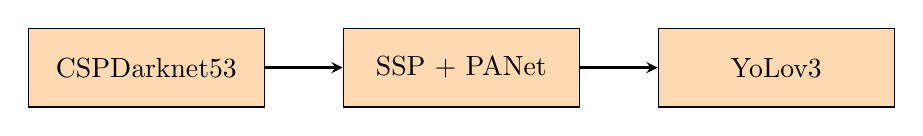
\begin{tikzpicture}[node distance=4cm]
    \node (backbone) [process] {CSPDarknet53};
    \node (neck) [process, right of=backbone] {SSP $+$ PANet};
    \node (head) [process, right of=neck] {YoLov3};
    \draw [arrow] (backbone) -- (neck);
    \draw [arrow] (neck) -- (head);
  \end{tikzpicture}
  \caption{The final architecture presented in the paper}
  \label{fig:final_arch}
\end{figure}

A couple of other combinations were derived but the FPS of the above combination superseded everything else.  A summary of the FPS values of a couple of other possibilities is given below. Now we are going to see some special sections of the architecture (but are not limited to) in detail which make it more efficient than YoLov3.

\begin{table}[h]
 \def\arraystretch{1.5}
 \centering
 \caption{Neural network parameters for image recognition for $512 \times 512$ network resolution}
 \begin{tabular}{|c|c|c|c|c|c|}
  \hline
  Backbone model & Receptive field size & Parameters & Average layer size & BFLOPs & FPS\\
  \hline
  CSPResNext50 & $425 \times 425$  & $20.6$ mn & $1058$ K & $31$ & $62$                   \\
  \hline
  CSPDarknet53 & $725 \times 725$ & $27.6$ mn & $950$ K & $52$ & $66$                        \\
  \hline
  EfficientNet & $1311 \times 1311$ & $12$ & $668$ K & $11$ & $26$                        \\
  \hline
 \end{tabular}
 \label{tab:mccons}
\end{table}


\subsubsection{Cross Stage Partial connection (CSP) \cite{Wang_2021_CVPR}}
In any large neural network-based architecture, it is common for the last and the second to last layers to lose out on a lot of contextual features seen by the initial layers. A way out of this is to introduce the concept of skip connections so that the backpropagation of gradients to the initial layers can be done easily. DenseNet was initially considered for this but it had skip connections between every other layer which proved to be inefficient. So, the researchers stuck with their initial choice of CSPResNext50 and the CSPDarknet53 as far as the architecture is concerned. Following is an illustration of the same.

\begin{figure}[h]
  \centering
    \includegraphics[scale=0.5]{chapter2/dense_architectures.png}
  \caption{The two possible dense architectures: DenseNet and CSPDensnet}
  \label{fig:dense_arch}
\end{figure}

\subsubsection{Self-Adversarial Training (SAT)}
Deep learning is very much susceptible to \textit{adversarial data} so YoLov4 uses SAT to introduce precise amounts of perturbation in the data such that the predicted label stays the same as the original label. This helps it easily achieve good accuracies for even augmentations of simple images.

All these discussions prove the benefits and advantages of YoLov4 over YoLov3 and hence it's choice for the project. As always, all things are better quantified in a graph of mAP versus execution time as shown below.

\begin{figure}[h]
  \centering
  \includegraphics[scale=0.8]{chapter2/v3v4.png}
  \caption{YoLov4 vs other state of the art object detectors}
  \label{fig:v3_vs_v4}
\end{figure}


\section{Performance metrics for evaluating object detection models \cite{Koech2020}}  \label{metrics}

The entirety of this report deals with a large number of performance metrics used to evaluate a variety of ML/DL models. Some are popular and have been used to evaluate such models for a long time while some metrics are empirical in nature because their output is a combination of a variety of models dealing with different classes of inputs and outputs which are working together. However, we would be specifically discussing metrics used for the evaluation of the performance of object detection models in this section.
\subsection{Intersection over Union (IoU)}
This metric equals the amount of overlap between the ground truth denoted by $g_t$ and the predicted value by a particular model i.e. prediction denoted by $p_d$. It is to be noted that since this value is a ratio, it is a fraction consisting of numerator and denominator areas in appropriate units. Mathematically, it is given by
\begin{equation}
\centering
IoU = \frac{area({g_{t}}\cap{ p_{d }})}{area({g_{t}}\cup{ p_{d }})}
\end{equation}
As it is very obvious for any arbitrary situation $0 \leqslant $ IoU $\leqslant 1$ wherein $0$ corresponds to a null overlap and $1$ corresponds to a full overlap. However, in almost all ML/DL models we don’t go for such strict definitions rather we define what we call the IoU at $\alpha$ (or abbreviated as IoU@$\alpha$). This means any value of IoU $\geqslant \alpha$ is considered a true positive whereas any value otherwise is considered a true negative. \par

Before we go ahead and define the next important metric we need to know a couple of different terms as stated below:
\begin{itemize}
 \item \textbf{Precision} – The degree to which a model can identify only the relevant objects. It is simply the ratio of true positives and all the detections made by the model. It is given by
\begin{equation}
\centering
P = \frac{True \ positives}{All \ detections \ made \ by \ the \ model}
\end{equation}
 \item \textbf{Recall} – The degree to which the model can detect all true positives amongst all ground truths. Mathematically, it is the ratio of the number of true positives and all ground truths and is given by
\begin{equation}
\centering
R = \frac{True \ positives}{All \ ground \ truths}

\end{equation}

\textbf{A good model has a high precision as well as high recall}.

 \item \textbf{Precision–recall curve} – It is simply the plot of the variation of precision and recall against the variation of confidence values. A good model will give high precision values even when confidence is varied significantly.
 \item \textbf{Average precision} – When the area under the precision-recall curve is calculated at the IoU@$\alpha$ threshold then we get this value. Formally, it is defined using the following integral.
\begin{equation}
\centering
AP@\alpha = \int\limits_{0}^{1} p(r) \ \mathrm{d} r
\end{equation}

\end{itemize}

Now we are at a stage where we can understand the next important metric

\subsection{Mean Average Precision (mAP)}
For each class, the average precision as defined above is calculated. This roughly translates to No. of average precision values $\approx$ No. of classes. When the average of these average precision is taken we get what we know as the mean average precision. For $n$ classes we can simply calculate it as follows:
\begin{equation}
\centering
mAP@\alpha = \frac{1}{n} \sum_{i=1}^{n} AP_{i}
\end{equation}


\section{Guidelines for a good YoLo project} \label{mod_guides}
The following rules for a good project using YoLo are mere \textit{thumb – rules} and are not some strict guidelines to be followed and should be evaluated on a case to case basis for every project. Additionally, it should be noted that such rules may not be applicable for implementation in every object detection project. The following rules are bifurcated into those undertaken during the training and those in the testing (detection) phase.

\subsection{For training}

\begin{enumerate}
  \item The values of {\fontfamily{qcr}\selectfont random} should be set to $1$ in your  {\fontfamily{qcr}\selectfont .cfg} file which allows training for multiple image or video resolutions simultaneously.
  \item Every distinct object that is liable for detection must have an appropriate label in the dataset.
  \item Precision may be increased by keeping the height and width of images or video frames as a multiple of $32$.
  \item The training dataset should be such that every object to be detected corresponds to an exactly similar object in the training dataset. Similarity should be in terms of size, no. of classes to be detected ($c$), overall spatial orientation, overall illumination, augmentation (if any) etc. \par

  If the size of the training dataset is $N$ and the no. of classes is stated as above then training must run for at least $Nc$ iterations.
  \item Training datasets should have as many \textbf{positive} examples as there are \textbf{negative} examples (i.e. images which don’t have any object to be detected). When the detection or testing run is executed, such negative examples shall return no bounding boxes. These ensure an equal sensitivity of the model to both types of images as well as eliminate a lot of post-processing operations.
  \item Sometimes it is desirable to run your detections with the {\fontfamily{qcr}\selectfont -show\_imgs} option at the end so that it can be manually verified whether the predicted bounding boxes are correct or not. Seeing the detections and detecting some anomaly could be a direct implication of training runs going wrong or some inherent problem in the dataset.
\end{enumerate}


\subsection{For testing or detection}

\begin{enumerate}
  \item Increase network resolution in the same way as mentioned in 1. c.
  \item It should be noted that retraining is not required in the event of loss in your dataset or any other unintended corruption. Only the \textit{darknet} command should be available which can be used to perform detections using the pre-trained {\fontfamily{qcr}\selectfont .weights} file which was trained on the $416 \times 416$ resolution images.
  \item To further enhance the accuracy, dataset training must proceed onto higher multiples of  $32$ such as $608 \times 608$ or $832 \times 832$. In the event of a memory overflow ({\fontfamily{qcr}\selectfont Out of memory}), {\fontfamily{qcr}\selectfont subdivisions} in your {\fontfamily{qcr}\selectfont .cfg} file must be increased from $16$ to $32$ to $64$ and so on.
\end{enumerate}

\chapter{Methodology and development} \label{chapter3}

\chapter{Deployment in production} \label{chapter4}

\section{ML models in production}


Rarely do data science projects in academia ever reach production and into a streamlined architecture. There are several reasons which prevent it from happening so. Indeed statistics say that roughly $87\%$ of all data science projects never make it into production \cite{vb2019}.  There are so many issues that hamper companies and developers to do so. We will be discussing only a couple of them here. \par

It is seen that even in professional work environments, data scientists rarely have the access to the right kind of data. Either they face issues due to the \textbf{network policy} in a corporate environment or the data is simply out of their reach. Another issue that quickly catches up with this issue is that a large amount of data already exists in the public domain, however, it is unorganised and exists in a completely unstructured format. More precisely, the data exists in a mixture of various formats namely structured, unstructured and semi-structured data. Such types of data need to go through rigorous cleaning and upkeep mechanisms, the process flow of which is sometimes difficult to figure out. Along with these two issues comes a very humane issue regarding the very basis of how data scientists typically work: in an individual manner. However, putting data models into production happens to be the best example of a collaborative effort by a company and hence can’t be single-handedly attempted by an individual. Apart from that technical issues of choosing the right framework, selecting the appropriate storage setup for your data and models etc. continue to exist.\par

We realise that the problems discussed above are as technical as they are humane. All these requirements gave rise to a completely new role for an MLOPs engineer \cite{Odegua2020}

Fortunately, for this project, the deployment of the data models falls within its current scope. All the ML models which would be trained and tested would be loaded onto the proprietary \textbf{Ezmeral MLOPs platform by HPE}. The servers for the same reside alongside the required hardware resources on SEBI’s internal servers. Doing this (without going into the details) would make the entire process streamlined i.e. the process of uploading videos, and training models on new data as soon as it is available and at the same time would decrease the manual work involved while doing so. As soon as the deployment has been completed, whether for all the NEWS shows or even a few of them, the internal server would be able to serve requests from within the organization domain (POST methods with JSON body) and at the same time would be able to abstract all the complex code and scripts running in the background. Following is an illustration of the complete MLOPs lifecycle which is allowed by (or within) the Ezmeral MLOPs platform.

\begin{figure}[h]
  \centering
  \includegraphics[scale=0.9]{chapter4/ML_DL lifecycle.jpeg}
  \caption{Machine learning lifecycle in production}
  \label{fig:ml_dl_cycle}
\end{figure}

\section{A two-part deployment}

This section deals with the needs of SEBI requiring a two-part deployment and the importance of each type in detail.

\subsection{Ezmeral MLOPs} \label{ezmeral}

The remaining part of this section deals with a proper \textit{yet brief} study of the very exhaustive HPE Ezmeral official documentation to send these models to production. It should be noted that the Ezmeral platform is quite large and only a small part of it deals with proper MLOPs. An even smaller part concerns the project at hand due to the nature of the license procured by the governing organization (SEBI) i.e., we won’t be looking at complicated use cases involving Kubernetes clusters or anything similar. Only the relevant parts of the study have been mentioned below.
The entire Ezmeral architecture looks something as follows. \newpage

\begin{figure}[h]
  \centering
  \includegraphics[scale=0.7]{chapter4/ML_DL solution.jpeg}
  \caption{The Ezmeral MLOPs solution}
  \label{fig:ml_dl_sol}
\end{figure}

As per the above architecture following are some sequential steps to be followed while deploying a model to production: \cite{Chiang2020}

\begin{enumerate}
  \item Usually, the process begins with the setting up of a proper environment within the Ezmeral cluster. This involves the allocation of appropriate system privileges to various users in a system. Since it’s a server-based system, it is customary to have multiple users and to allocate their various levels of access to the system. The platform admin is responsible for this job. After doing so, various required apps (which are essentially docker images) relevant to the application may be downloaded.
  \item After this the project repository is created and appropriate data loaded. This may include pre-written scripts, datasets for training and testing as well as pre-trained models (which may be improvised later on). It should be noted that that every one among those things belongs to persistent storage and there would be no data loss in the case of a server outage.
  \item Followed by this an appropriate training cluster is to be allocated for a given project: the software concerned currently allows bindings with a variety of CPUs and VCPUs (called flavours). These have different specifications in terms of memory and speed.
  \item  This is followed by actual programming in a Jupyter notebook attached to this cluster wherein after the initial phase, dedicated training regimes would utilise these cluster resources.
  \item  Followed by the creation and training of a model within the attached Jupyter notebook, the programmer is expected to \textbf{register the model} for further training at a later stage. At this point, the model gets stored in the persistent section of the Ezmeral cluster could be utilised later for further and more advanced training. Beyond this, in typical industrial use cases (such as this), scheduled scripts are just run which re-run this training procedure as many times as required.
  \item  After a successful model registry, the server should be in a position to serve requests from the expected domains (in this case only requests from within the SEBI domain). To do so, again appropriate CPUs/VCPUs are assigned to balance the load, serve REST API requests etc.
  \item It should be noted that only the scoring script written in Python is run for any given request with the appropriate arguments provided in the JSON request. Hence, apart from the complex steps described above, the entire process boils down to a single Python script execution at the end. \par

        \textbf{Followed by this the server is ready to respond to a variety of requests from the concerned domain}.
\end{enumerate}

This concludes the discussion on the entire ML – DL workflow to be used on the Ezmeral MLOPs platform. However, we didn’t go into details about server availability in terms of uptime or downtime nor did we go into the details of the amount of storage available to SEBI who has purchased this platform. It so turns out that although this discussion was not done, this is one of the most principal aspects of the deployment. \par

The Centos VM on top of which the entire Ezmeral cluster resides is used for a lot of tasks \textbf{\textit{apart from the one described above}}. This leads to a low-frequency and high-latency solution which is not good for any MLOPs service use case. Therefore, it was decided that although this setup would be developed in its entirety, this is reserved for only single-usage queries for obtaining the output to only specific videos at a time. \par

The greater requirements at the time were to perform massive batch processing workflows which are freely running and would manage to process several hundreds of videos in sequence. Hence, the second part of the deployment concerns a single VM workflow as described in the following section.

\subsection{Single VM workflow} \label{vm}

To overcome the single-usage and as-in-required constraints described above, we have decided to go for an \textbf{automation script} that calls the main Python script repeatedly to process the bulk of videos that are in turn fetched from a remote server. In this case, it is SEBI’s Datalake server. \par

The concerned setup involves a Linux VM running Centos 8.2 which is relatively ideal and is not involved in unnecessary workflows apart from the concerned one. All the required assets i.e. code (the main Python script \textit{aka} the scoring script in the above section), data (ML models and image templates or masks) and excel files containing a readymade listing of companies are to be made available on the VM. Apart from this the automation script (which is also written in Python) resides on the VM. The logic inside the automation script is segmented into the following parts.

\begin{itemize}
  \item Connecting and disconnecting to the remote server.
  \item Fetching and sending files from and to the remote server respectively.
  \item Performing normal command-line actions on the VM on which it resides: running the Python scoring script repeatedly with command-line arguments and deleting unnecessary files after a single execution run.
  \item Show the current stage of the workflow which is under progress and display a final summary of the total no. of videos that have been processed successfully and(or) the number of videos that have failed.

\end{itemize}

We shall elaborate on the last point a little further. Execution of the scoring script on a single video file leads to the production of a single CSV file at the location of the VM and produces a very large log file wherein the entire output of the script was redirected. The CSV file and the log file need to be sent back to the remote server followed by which they are to be deleted from the VM. Since the video file also doesn’t have any further use, it is also deleted subsequently. The correct order in which this is to be done is elaborated in the last section of this chapter as a guideline for similar scenarios. Upgrades have been planned for this workflow as detailed further in section \ref{future}.


\section{Overall software flow}

\textbf{Step 1}: Open a connection with the remote SEBI Datalake server. Exit the program if a timeout error occurs with an appropriate exit code. \\[5mm]
\textbf{Step 2}: Fetch the next video file in sequence from the remote server. \\[5mm]
\textbf{Step 3}: Run the Python scoring script on the same. A log file will be created as a result of this. And a CSV file only if the execution is successful. \\[5mm]
\textbf{Step 4}: Delete the video file. \\[5mm]
\textbf{Step 5}: Send a copy of the log file to the server and delete its instance from the VM. \\[5mm]
\textbf{Step 6}: If \textbf{Step 3} was successful, send a copy of the generated CSV file to the remote server and delete its instance from the VM.



The entirety of the above process flow has been shown on page \pageref{fig:soft_process_flow}.

\begin{figure}[h]
  \centering
  \begin{tikzpicture}[node distance=2cm]
    \node (start) [startstop] {Start};
    \node (conn) [process, below of=start, yshift=0.5cm] {Open connection with remote server};
    \node (dec1) [decision, below of=conn, yshift=-1.5cm] {Connection timeout?};
    \node (stop1) [startstop, right of=dec1, xshift=3.5cm] {Stop};
    \node (fetch) [process, below of=dec1, yshift=-1.5cm] {Fetch video file from server};
    \node (exec) [process, below of=fetch, yshift=0.5cm] {Execute scoring script};
    \node (del_video) [process, below of=exec, yshift=0.5cm] {Delete video file};
    \node (send_del_log) [process, below of=del_video, yshift=0.5cm] {Send log file to server and delete from VM};
    \node (dec2) [decision, below of=send_del_log, yshift=-1.5cm] {Successful execution?};
    \node (stop2) [startstop, right of=dec2, xshift=3.5cm] {Stop};
    \node (send_del_csv) [process, below of=dec2, yshift=-1.5cm] {Send CSV file to server and delete from VM};
    \node (stop) [startstop, below of=send_del_csv,yshift=0.5cm] {Stop};
    \draw [arrow] (start) -- (conn);
    \draw [arrow] (conn) -- (dec1);
    \draw [arrow] (dec1) -- node[anchor=west] {No} (fetch);
    \draw [arrow] (dec1) -- node[anchor=south] {Yes} (stop1);
    \draw [arrow] (fetch) -- (exec);
    \draw [arrow] (exec) -- (del_video);
    \draw [arrow] (del_video) -- (send_del_log);
    \draw [arrow] (send_del_log) -- (dec2);
    \draw [arrow] (dec2) -- node[anchor=west] {Yes} (send_del_csv);
    \draw [arrow] (dec2) -- node[anchor=south] {No} (stop2);
    \draw [arrow] (send_del_csv) -- (stop);
  \end{tikzpicture}
  \caption{Overall software process flow represented as a simple flowchart}
  \label{fig:soft_process_flow}
\end{figure}



\section{Guidelines for deployment}

This section presents a set of guidelines for the two types of deployment detailed in sections \ref{ezmeral} and \ref{vm}.

\begin{enumerate}
\item Concentrate on three fundamental aspects of the MLOPs solution namely how the data is going to be stored and retrieved, what frameworks are applicable and(or) available for your job and finally the iterative processes involved in your MLOPs solution \cite{Odegua2020}.

\item Condense your workflow to a few specific data types in which your input data is to be stored e.g. .mp4 files as in this case.

\item Be careful with the amount of data to be stored: look for the best solution fitting your budget.

\item Classify whether you would be dealing with batch workflows or predictions by your ML models in real-time as detailed in sections \ref{vm} and \ref{ezmeral} respectively as this shall greatly affect your outcome.

\item If you are dealing with batch workflows as in section \ref{vm}, the order of fetching and deleting files is paramount. Classify files into input, files produced irrespective of the status of the result and files produced only on successful execution. Order them by size and the sequential points of failure. Delete the largest input file(s) first followed by sequential cycles of sending files to the remote server and deleting them.

\chapter{Results and discussions} \label{chapter5}

The following subsections shall discuss in detail, a variety of important comparisons which affect the project work, a brief overview of the methodologies learned, deviations from the ideal case (if any) and a creator’s road map for implementation of a similar project and other moderately or less important details. It also has a section for the work which is being currently done at SEBI to improve the existing system. The initial two sections deal with metrics of accuracy and execution time across two different bases for comparison while the section that follows discusses why the metrics are chosen and defined as they are. \par

\section{Comparison between OCR models}

Both Tesseract and EasyOCR are sophisticated OCR engines and are available as open-source in their default versions. However, there exists a large number of differences in how they have been developed. While Tesseract \cite{Google2015} happens to be a quite superior alternative right from the beginning which can use even PDF files as input apart from the standard images, it turns out that there doesn’t exist any suitable interface with common programming languages (such as Python) which leads to a lot of problems. The first and foremost problem is that Tesseract needs to be set up in a way similar to how a particular program is set up on a remote server i.e. the only link between a program using Tesseract and the actual engine is the file path. Customisations can be done nonetheless, but are difficult to implement due to the lack of a high-level interface. This leads directly to another issue: the Ezmeral MLOPs platform is set up on a legacy Centos 7.5 virtual machine cluster and won’t allow arbitrary software to be installed in it due to the presence of an enterprise-grade security architecture.  So it may be the better OCR engine in general, however, this use case is unsuitable for it.\par

EasyOCR offers as many capabilities \cite{Jaided2020} as Tesseract (sans the direct processing of PDF files) and has a high-level library directly available for use in Python. This means that no preliminary server like set-up needs to be done to access the OCR engine, rather everything is on board once the program and all its imported modules are loaded onto memory. Hence, EasyOCR was chosen as the OCR for this project. \par

It should be noted that EasyOCR is a ready-to-use OCR that is invariant to colour images while the Tesseract documentation does say things about providing a greyscale image as input. This feature alone avoided a lot of extra image processing operations within the codebase. After using EasyOCR, the following changes took place:

\begin{itemize}
 \item The size of the codebase was greatly reduced.
 \item The execution time dropped significantly.
 \item Major improvements were not visible in accuracy although EasyOCR still managed to perform better.
\end{itemize}

Amongst all decoded values at the end of a particular run, the following results were obtained and are summarised below.

\begin{figure}[h]
  \centering
  \includegraphics[scale=0.7]{chapter5/barchart.png}
  \caption{Comparison of Tesseract and EasyOCR for a sample $30$ minutes telecast}
  \label{fig:easy_vs_tess}
\end{figure}

Still, EasyOCR (and the project) benefits even further from a possible change in hardware configuration which is detailed in the following section.


\section{Comparison between hardware architectures}


\section{Accuracy, empirical accuracy and execution time}

A lot has been discussed about the various performance metrics used to evaluate object detection models in section \ref{metrics}, however, we still stick to the concept of simple empirical accuracy in the above two sections. The reason for the same is that there are multiple ML/DL models which are involved in this project. Each model has been designed (or is being used) to complete only a specific task amongst a large number of tasks that are to be executed sequentially. Each task involves different kinds of data and hence produces different kinds of output. \par

A simple e.g. being that the YoLo models discussed throughout the report output a set of mixed values as given in section \ref{brief_discuss} after taking in an image as an input. However, the OCR models that follow require an image as an input, but produce a textual output (i.e. of string datatype). These models within them have two deep learning models i.e. a text detection and a language model in a cascaded fashion out of which only the former receives an input in the form of an image while the second model deals with textual input and output. \par

Each of these models named above has its own set of accuracy metrics which may be discussed however, they would be irrelevant to the final output of the project. Hence, we have stuck to the concept of simple empirical accuracy which is defined by the set of values obtained at the end from the OCR and summarised in the CSV file and is defined as follows

\begin{equation}
\centering
A_{e} = \frac{No. \ of  \ NA \ values \ in \ the \ CSV}{Total \ no. \ of \ values \ in \ the \ CSV }

\end{equation}

Measuring execution time remains the same i.e. in seconds although at a couple of places wherein the execution time is large, seconds have been replaced by larger units of time.
\section{Future work}

The current system can be improvised in two different areas as given below.

\subsection{Accuracy and efficiency}

The current system does filtering at only the FPS rate which manages to reduce the number of frames under consideration to a much smaller value (a $25$\textsuperscript{th} of it to be precise). However, as we have seen in chapter \ref{chapter3}, the frame selection is still not inherently intelligent and still leads to the production of  $ \approx 1400$ frames on an average, amongst which frames would be manually selected for annotation. \par

Theoretically, we can say that for the problem statement at hand; there exists a program $P$ that extracts and processes exactly $N$ frames such that the total no. of recommendations being made is $R \leqslant N$. \par

To do so we can use an adaptive frame extraction algorithm \cite{adapt} which shall extract only the frames which are important to us. This method is based on matching histograms of successive frames, a correlation that exists amongst their colour channels, etc. This shall greatly reduce the number of frames to be processed at a time (apart from the already existing FPS rate filtering). This method, however, could be tending to fail because similar-looking frames need not be redundant to us just because they appear close to each other in the actual video. In that case, we can go for an alternative approach wherein the frame numbers are output according to a simple implementation of any multi-output regressor \cite{ Brownlee2020}. Since there could be inherent inaccuracies in the training of the same, we can use a spreading factor $\delta$ which shall extract keyframes starting from ${f}_{k} - \delta$ to ${f}_{k} + \delta$ instead of just the frame $f_k$.

\subsection{Usability}

Currently, a two-part deployment and its necessity are deemed to be confusing to many SEBI officers who work in the surveillance department and don’t have any prior programming knowledge. Both these deployments could be integrated into a single native cross-platform desktop app developed either using \href{https://riverbankcomputing.com/software/pyqt/intro}{PyQt} or \href{electronjs.org}{Electron} which shall have an intuitive front end design and the same set of calling scripts as its backend. This shall help concerned officers keep track of ongoing workflows as well as use them when required without interfering with ongoing batch workflows and being aware of the complexity of the ML/DL code behind it.

\chapter{Conclusions} \label{chapter6}

The various recommendations being made in NEWS shows were successfully detected (within tolerable error limits across a large size of input data), extracted and analysed for anomalies in the concerned process.  The input to the program script was simply the video file itself and the telecast date (which was reflected as it is in the last column). The summarised data was available to the end-user in either an excel file or CSV file for further analysis. The final summarised data contained important fields like the \textbf{Name of the analyst}, the \textbf{share/stock} regarding which recommendation was being made: its \textbf{name} as well as its \textbf{listing symbol} in the appropriate exchange, the \textbf{actual recommendation} being made (buy, sell or hold), the \textbf{target price} and the associated \textbf{stop loss}.  A total of eight NEWS shows were processed in this manner wherein only a single NEWS show was skipped due to the lack of recommendations being made in the video dataset available to us. \par

As stated earlier in chapter \ref{chapter4}, the deployment of the above ML/DL models was parallelly done onto two separate systems, namely the HPE Ezmeral MLOPs server for single usage low-frequency requests and on a separate Linux virtual machine for large free-running batch processing workflows which would keep on running a single script continuously on a large dataset. \par

I got to learn a lot of things regarding machine learning, deep learning for computer vision, functioning of OCR engines, MLOPs deployment in different environments and as well as different guidelines which are to be followed for gathering a video dataset (e.g. sampling at FPS rate, annotating a dataset, partitioning the dataset properly etc.) and processing it accordingly for further analysis. Overall it turned out to be an entire knowledge enriching experience spanning a multitude of domains.




\newpage
\printbibliography
\addcontentsline{toc}{chapter}{Bibliography}


\end{document}
